


\chapter{Process Management and Scheduling}
Data is coming in at different, independent rate from sensors and is produced asynchronously from internal processing elements.
For certain processes, processing the incoming data as quickly as possible is key, however, this is challenging for several reasons:
1) a process may subscribe to multiple, independent streams with asychronized report schedules and 2) interpolated values
should be avoided to minimize prediction inaccuracies in interpolated values.  Therefore, a process actually wants all the freshest
data from all the streams they are subscribing to, while minimizing the average time that the data for each respective stream has 
been waiting in the buffer.

\section{Process Management}
%\input{external_tex/streamfs_aggregation/}
Sensor data is fundamentally challenging to deal with because much of it must be cleaned before it can be processed.  For example,
it is not uncommon to receive readings that is out of operational range, that is erroneous with respect to the previous observed trend,
or to stop receiving readings altogether.  This implies the need for processing jobs to provide a level of filtering over the raw streams.
Once the data is cleaned, it is typically consumed more sophisticated processes that aggregate the information or use it for control
of the space or equipment.  We provide the mechanisms for handling both classes of processing jobs with our process management layer.
In the next section we will discuss our process management layer and how users can both submit jobs to StreamFS for management or link
their own external processing elements so that they can be managed through StreamFS but run outside of StreamFS.


% \section{Processing Pipelines and Management}
% \section{Entity Relationships}

\section{Internal Processes}
Internal processes are jobs submitted to StreamFS that are written in Javascript and managed within a StreamFS cluster.

\section{Mapping OLAP to ERG}

\begin{itemize}
\item Introduction to OLAP.
\item Explanation of ERG in StreamFS.
\end{itemize}
Online analytical processing (OLAP) is a processing layer that provides summurization of data
from a set of underlying data repository (date warehouses).  Traditionally, OLAP is used to process
business data.  Business data summurization allows an analyst ask targetted questions about aggregates 
and trends in their data.  The data is typically multidimensional in nature and operations can be performed with
respect to those dimensions and their inter-relationship.

\subsection{Measures, Dimenions, and Levels}

\subsection{Operations: drill-down and roll-up}

\subsection{Operations: slice and dice}

\subsection{Operations: pivoting}
\section{Dynamic Aggregation}
\label{sec:dynagg}
Dynamic aggregation combines the underlying entity-relationship graph with in-network aggregation.  It treats
each node in the graph as a potential point of aggregation on a particular data type.  For example,
if we need to compute aggregates of \emph{KW} data and we declare the node for a particular room as
the point of aggregation, we accept data from all children of that node that, whose units are in \emph{KW},
and add the streams together over pre-defined window size or pre-defined timeouts.

The scheme is hiearchical, so a node only accepts data from its children and only sends data to its parent.
StreamFS checks for cycles when before node insertion and prevents double-counting errors by only allowing 
aggregation-points that are roots of a tree that is a sub-graph of the entity-relationship graph.  In our deployment,
each view is a managed as an independent hierarchy.  So the hierarchy of \emph{spaces} is separate from
the \emph{inventory} hierarchy or the \emph{taxonomy} hierarchy.  This allows us to ask questions with a particular
view in mind, without conflict, and is a natural fit for our aggregation scheme.

\subsection{How it works}
Although there are different semantics applied to different node types at the application layer, StreamFS only knows
about two types of nodes: (1) default nodes and (2) stream nodes.  The main difference is that \emph{default} nodes
are not explicitly associated with data coming from a sensor and \emph{stream} nodes are.  Furthermore, default
nodes can have children, while stream nodes cannot.  In our application, meters are represented by default nodes
and each stream of data they produce is a stream node.

When an aggregation point is chosen and enabled, dynamic aggregation places a buffer at the node for the type
of data that should be aggregated.  If we want to aggregate \emph{KW} data, we specify the type and send an enable-aggregation
request to the node through an HTTP {\texttt POST} to the path for that node.  The flow of data starts at the leaves when
a stream node received data from a sensor through HTTP {\texttt POST}.  As data arrives it is immediately
forwarded upstream to the parent(s).  If a node that receives data from its children is an aggregation point it buffers
the data, otherwise it fowards it to its parent.

Ignoring the timeouts for now, lets imagine the parent is a point of aggregation and its buffer is full.  At this point
the parent separates data into bins for each source and cleans it for aggregation through interpolation.  The main
operation is to \emph{stretch} and \emph{fill} that data with linearly interpolated values.  The \emph{stretch}
operation orders all the timestamps in increasing order and for each bin (signal) interpolates the values using the
first (last) pair of data points.  If there is only a single data point, the stretch uses it as the missing value.
The \emph{fill} operation find the nearest timestamps that are less-than and greater-than the missing sampling time, 
uses their values to determine the equation of a line between them and interpolates the missing value using that equation.
Once this is done for each signal, the values are added together for each unqiue timestamp and the aggregated
signal is reported to the parent, where the operation occurs recursively to the root.
Figure~\ref{fig:aggtree} shows an illustration of its operation.  

%problem:  the buffer size has to increase exponentially up the tree, in order to not drop any values.
%solution: chuck the data into default-buffer sized pieces and parallelize the interpolation using the interpolated tasks technique


%FILL IN WITH REAL GRAPH
\begin{figure}[htb!]
\begin{center}
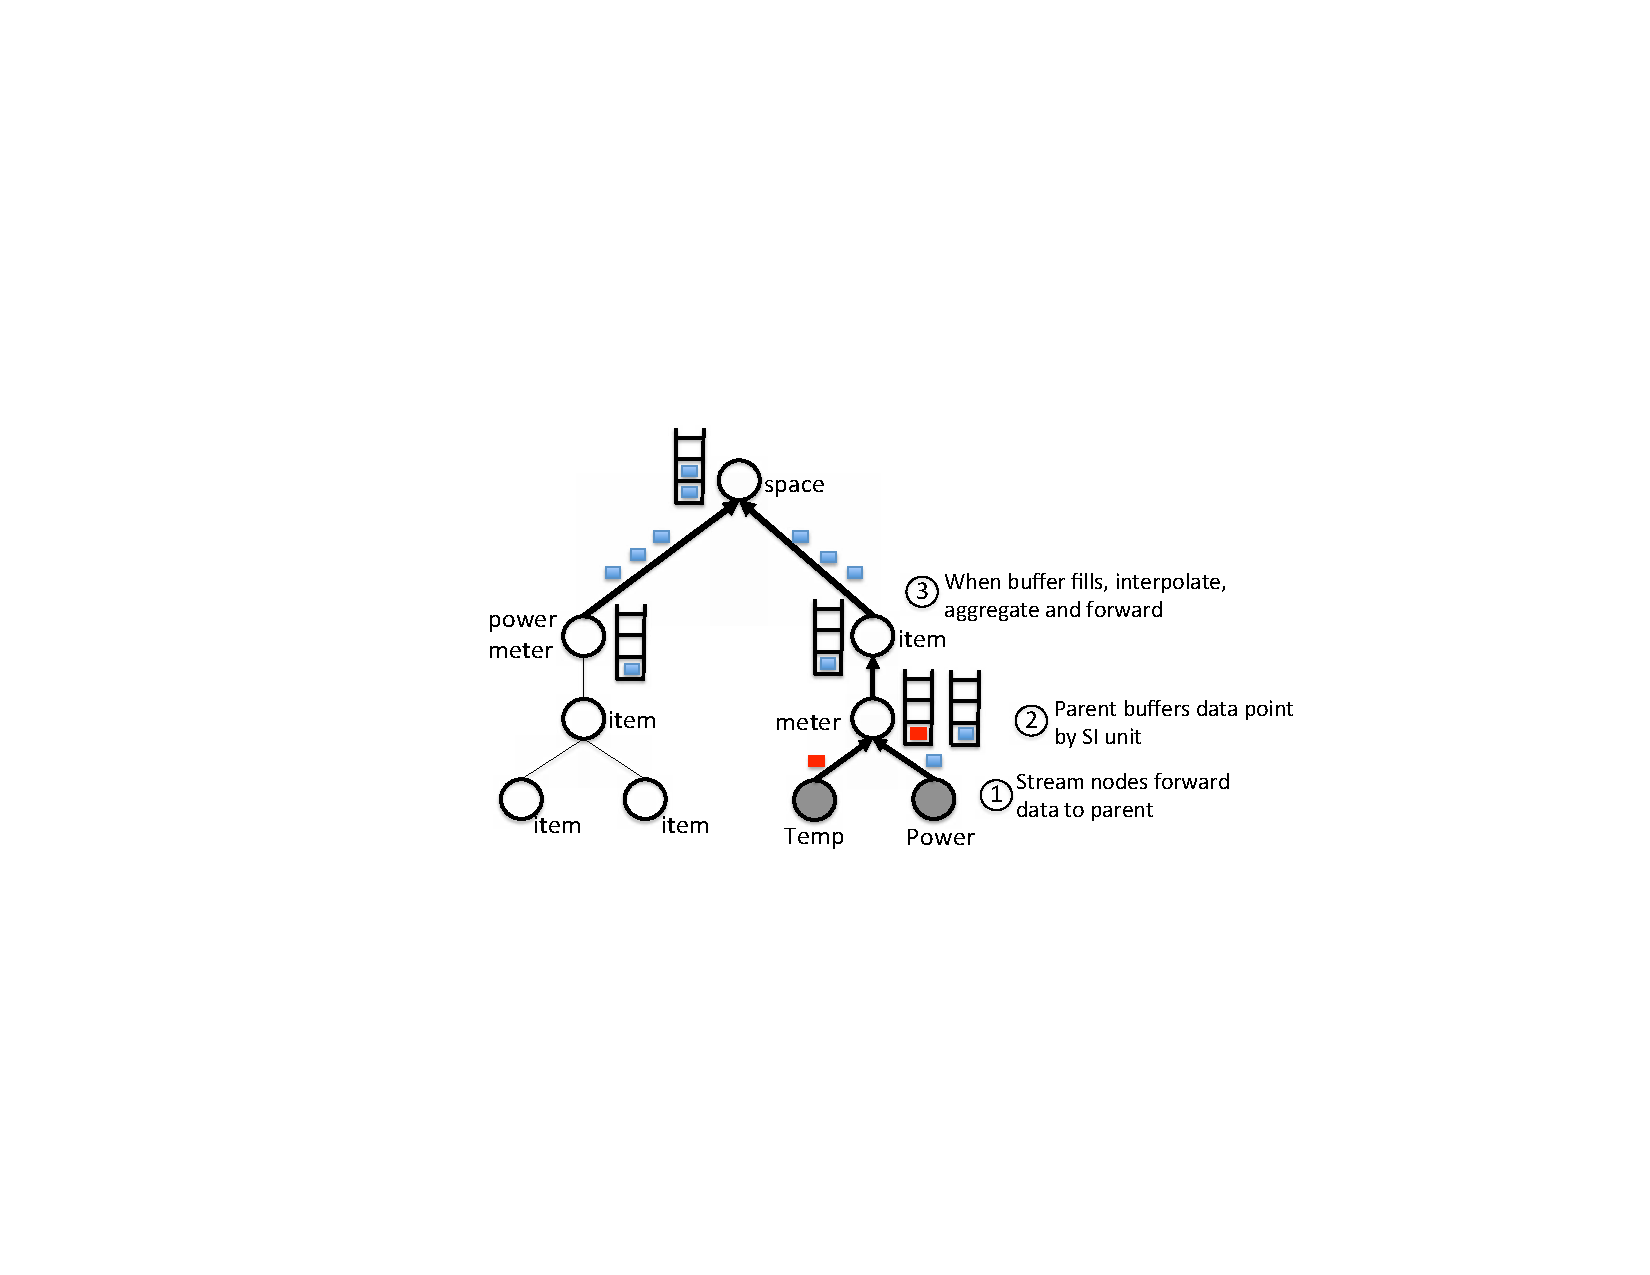
\includegraphics[scale=0.6]{figs/aggtree}
\caption{This shows an illustration of the aggregation tree used by \emph{dynamic aggregation}.  Data flows from 
the leaves to the root through user-specified aggregation points.  When the local buffer is full the streams
are separated by source, interpolated, and summed.  The aggregated signal is foward up the tree.}
\label{fig:aggtree}
\end{center}
\end{figure}

\subsubsection{Dealing with dynamics}
This approach deals with changes in the graph quite naturally.  All aggregation point deal only with local data, so
a node is only concerned about the children that give it data and the parent to send data to.  As objects in the environment
move from place to place and these changes are captured, the entity-relationship graph also changes to reflect the move.
This change in aggregation constituents is naturally accounted for in the aggregate.  If a child is removed,
it no longer forwards data to the old parent, therefore the aggregate will reflect that change.
Note, however, that changes in the entity-relationship graph are indistinguishable from energy-consuming items that have
been turned off.  For the purposes of aggregation, that is okay.

\subsubsection{Two scenarios}
We illustrate dynamic aggregation with a common usage scenario.  Imagine there are a number of people in a building,
each owning a number of plug-load applicances and a laptop.  Assume that when a person is in a room their laptop
is plugged in and when they leave the room they unplug their laptop and take it with them.  People come and go
throughout the day, changing the aggregate power consumption of the room and it happens.  In addition, some
of those people move to other rooms and plug their laptop in the new location.  As this happens, we will assume
all actions are being recorded in StreamFS.

%FILL IN WITH REAL GRAPH
\begin{figure}[htb!]
\begin{center}
\subfloat[Room 1 object and aggregate streams.]{%
            \label{fig:dynaggs1room1}
            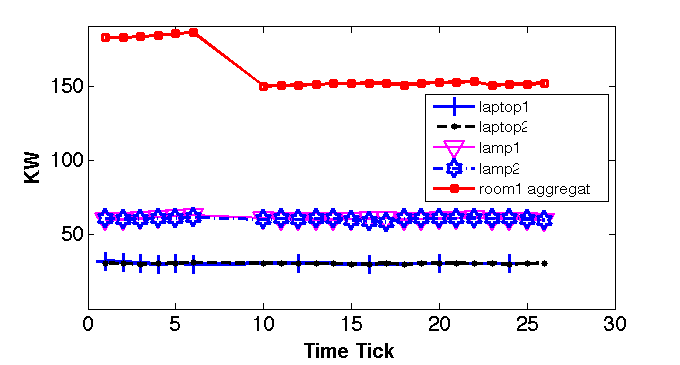
\includegraphics[scale=0.4]{figs/dynagg_scenario1_room1}
        }
\subfloat[Room 2 aggregate.]{%
            \label{fig:dynaggs1room2}
            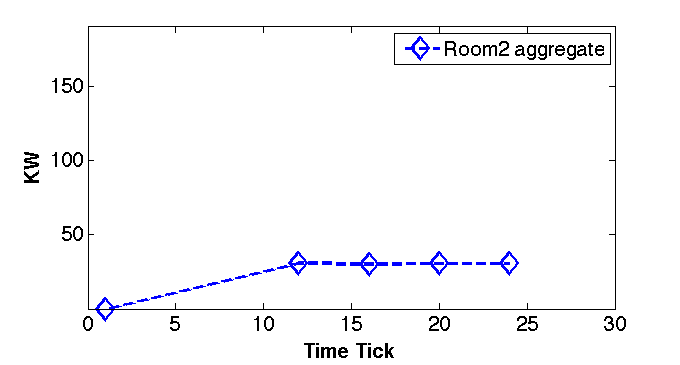
\includegraphics[scale=0.4]{figs/dynagg_scenario1_room2}
        }
\end{center}
\caption{
	The power consumes by a laptop in \emph{room 1} is shifted to \emph{room 2} a time t=7.  Notice the aggregagate drops in room 1
	while it rises in room 2.
     }%
\label{fig:multiroomagg}
\end{figure}

Figure~\ref{fig:multiroomagg} illustrate the aggregation results of that scenario.  Notice how...

% For demonstration lets have the user turn off on of their appliances when they leave as well.  This should cause that total
% room aggregate to drop, the person's personal aggregate to drop, but the other occupant's aggregate to remain
% the same.

% %FILL IN WITH REAL GRAPH
% \begin{figure}[htb!]
% \begin{center}
% 
\includegraphics[scale=0.39]{figs/blankbox}
% \caption{A room with items that belong to many users.  Person leaves with their item, aggregate falls.  Show aggregate.
% Person joins another room, aggregate in that room rises.  Show aggregate in the new room.  Compare before and after.}
% \label{fig:personaltotalagg}
% \end{center}
% \end{figure}

% Figure~\ref{fig:personaltotalagg} illustrate the results of the second sceanrio.  Note how...


\section{External Processes}

% \section{Designing for Horizontal Scalability}

%\section{Minimizing Data Time in Buffer}
\section{Maximizing Data Freshness}
Certain jobs only care about consuming the latest readings from their subscription streams.  They are willing to discard reading until two
conditions are met:

\begin{enumerate}
\item There is at least one data point from each stream in the subscription buffer.
\item The statelness factor is minimized within the immediate time window.
\end{enumerate}

This is of particular interest to controllers that need to make control decision based on the freshest data possible and can tolerate some variability
in the completion time of the control task.  It is also useful in analytical jobs that want to process the latest data from multiple streams while also
allowing some variability in the completion of the processing task.  Note, there's a fundamental tradeoff
between the staleness factor and variability of consumption.  It is sometimes better to wait for the next incoming data point than it is to use what
is currently in the buffer, as waiting will decrease the overall staleness factor.  Other times, it is better to consume the bufferred data immedaitely.
This causes a certain amount of variability in the delivery period to the control process.  However, for some applications, this is a reasonable tradeoff
to make.  Making use of the freshest data is desirable for minimizing errors, either in the control of a system or the calculation of some aggregate state.
Generally, the error grows with staleness, therefore the goal of this mechanism is to continuously minimize the error associated with staleness through
scheduling.


\begin{figure}[t!] %htbp
\centering
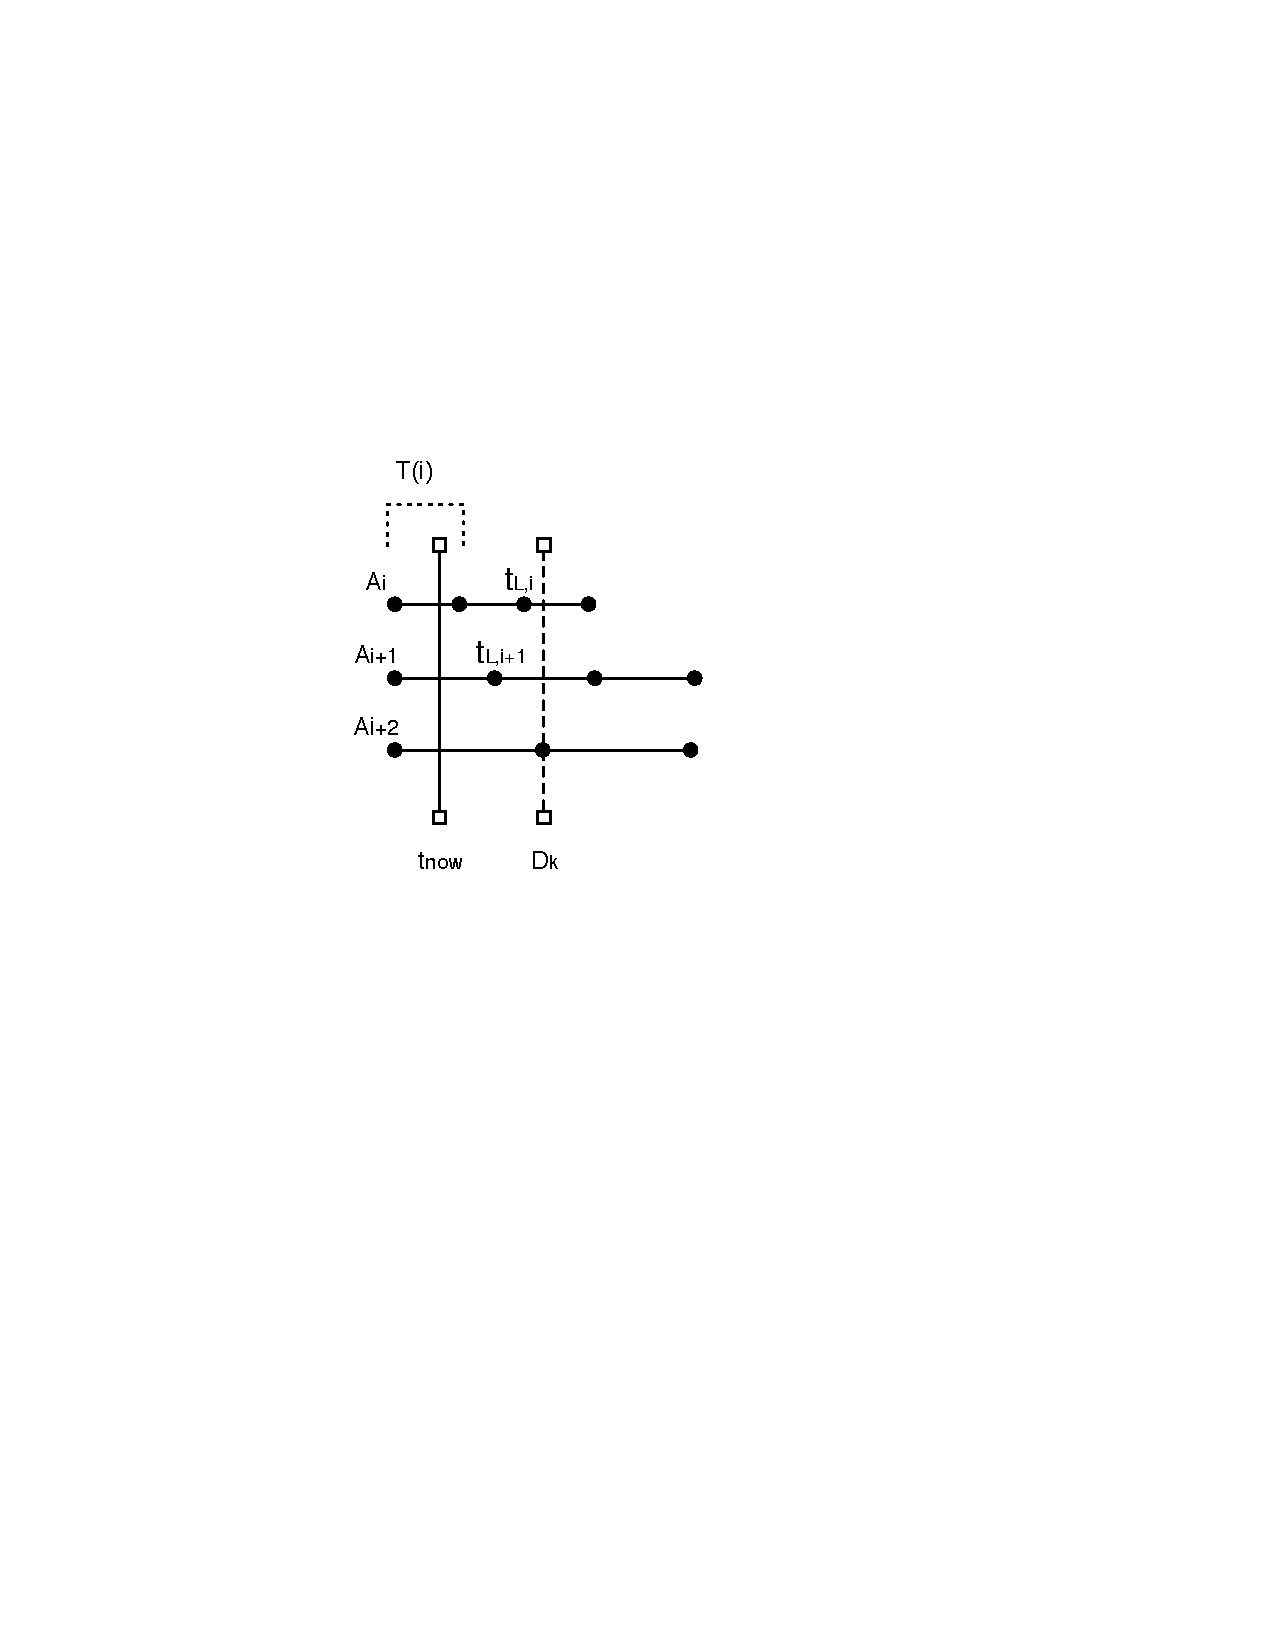
\includegraphics[width=0.75\columnwidth]{figs/min_buffer}
\caption{Multiple streams in a subscription and their associated parameters.}
\label{fig:min_buffer}
\end{figure}

Let $A_{i}$ be the arrival time of the last data point received from stream $i$ and $D_{i}$ be the arrival time for the next data point from stream $i$
and their relationship as described in equation \ref{eqn:deadline}, where $T(i)$ is the average period between the arrivals from stream $i$.

\begin{equation}
D_{i} = A_{i} + T(i)
\label{eqn:deadline}
\end{equation}


Periodically, our algorithm runs and checks if there is a data point for each stream in the subscription.  If so, the \emph{min\_buffer} algorithm runs 
and effectively decides whether to execute the job on the current buffer immediately or whether to wait until later, when the \emph{staleness factor} of
the buffer will be at a minimum.  This decision is driven by equation~\ref{eqn:later_better_condition}, whereby we find the next deadline, computed with
equation~\ref{eqn:last_deadline}, for each stream in the set and determine the staleness factor will be for the entire buffer if we wait until that deadline arrives.

\begin{equation}
t_{L,i} = A_{i} + \Bigl\lfloor \frac{D_{k}-A_{i}}{T(i)} \Bigr\rfloor T(i)
\label{eqn:last_deadline}
\end{equation}

If there is no deadline $D_{k}$ for some stream $k$ such that equation~\ref{eqn:later_better_condition} holds, then we execute now.  Otherwise we choose to wait
until $D_{k}$ for the stream whose next deadline minimizes the staleness factor of the buffer.


\begin{equation}
\sum_{i=1}^{k-1} D_{k} - t_{L,i} < \sum_{i=1}^{k} t_{now} - A_{i}
\label{eqn:later_better_condition}
\end{equation}

The algorithm is sketched our below.


\begin{algorithm}[h!]
 \SetAlgoLined
 Given a full buffer $b[n]$:\\
  \For{all elements in the $b$}{
  (1) Calculate the staleness of element $i$ and add to total stalness, $S_n$\;
  \For{all other elements in the buffer}{
  	(1) Determine the next report time $D_i$ for this element\;
  	(2) Determine the staleness of all the elements if we wait until $D_i$\;
  	(3) If it is the smallest staleness figure calculate, replace minimum cost, $S_l$.
  	}
  }
  \If{$S_l$ is less than $S_n$}{
  (1) Wait until later to consume\;
  \Else{
  (1) Consume now}
  }
 \caption{Staleness algorithm.}
 \label{alg:emd}
\end{algorithm}

\section{Experimental Results}

\begin{figure}[t!] %htbp
\centering
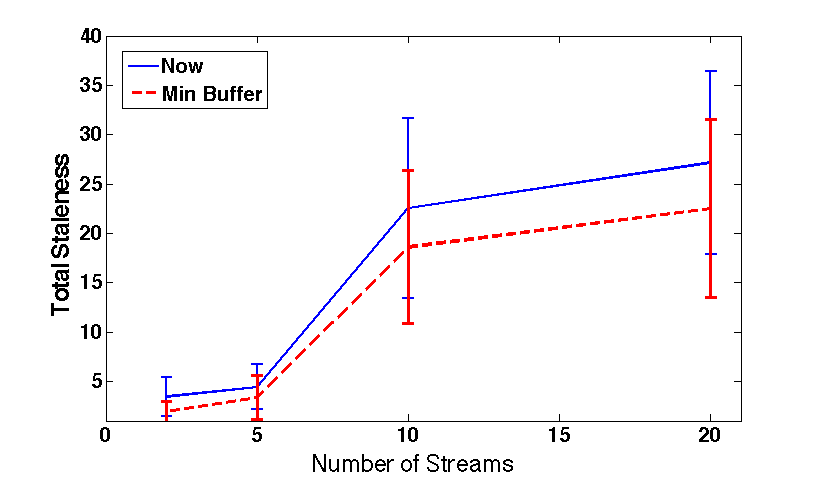
\includegraphics[width=0.9\columnwidth]{figs/staleness_vs_numstreams}
\caption{}
\label{fig:stalevsstreams}
\end{figure}

\begin{figure}[t!] %htbp
\centering
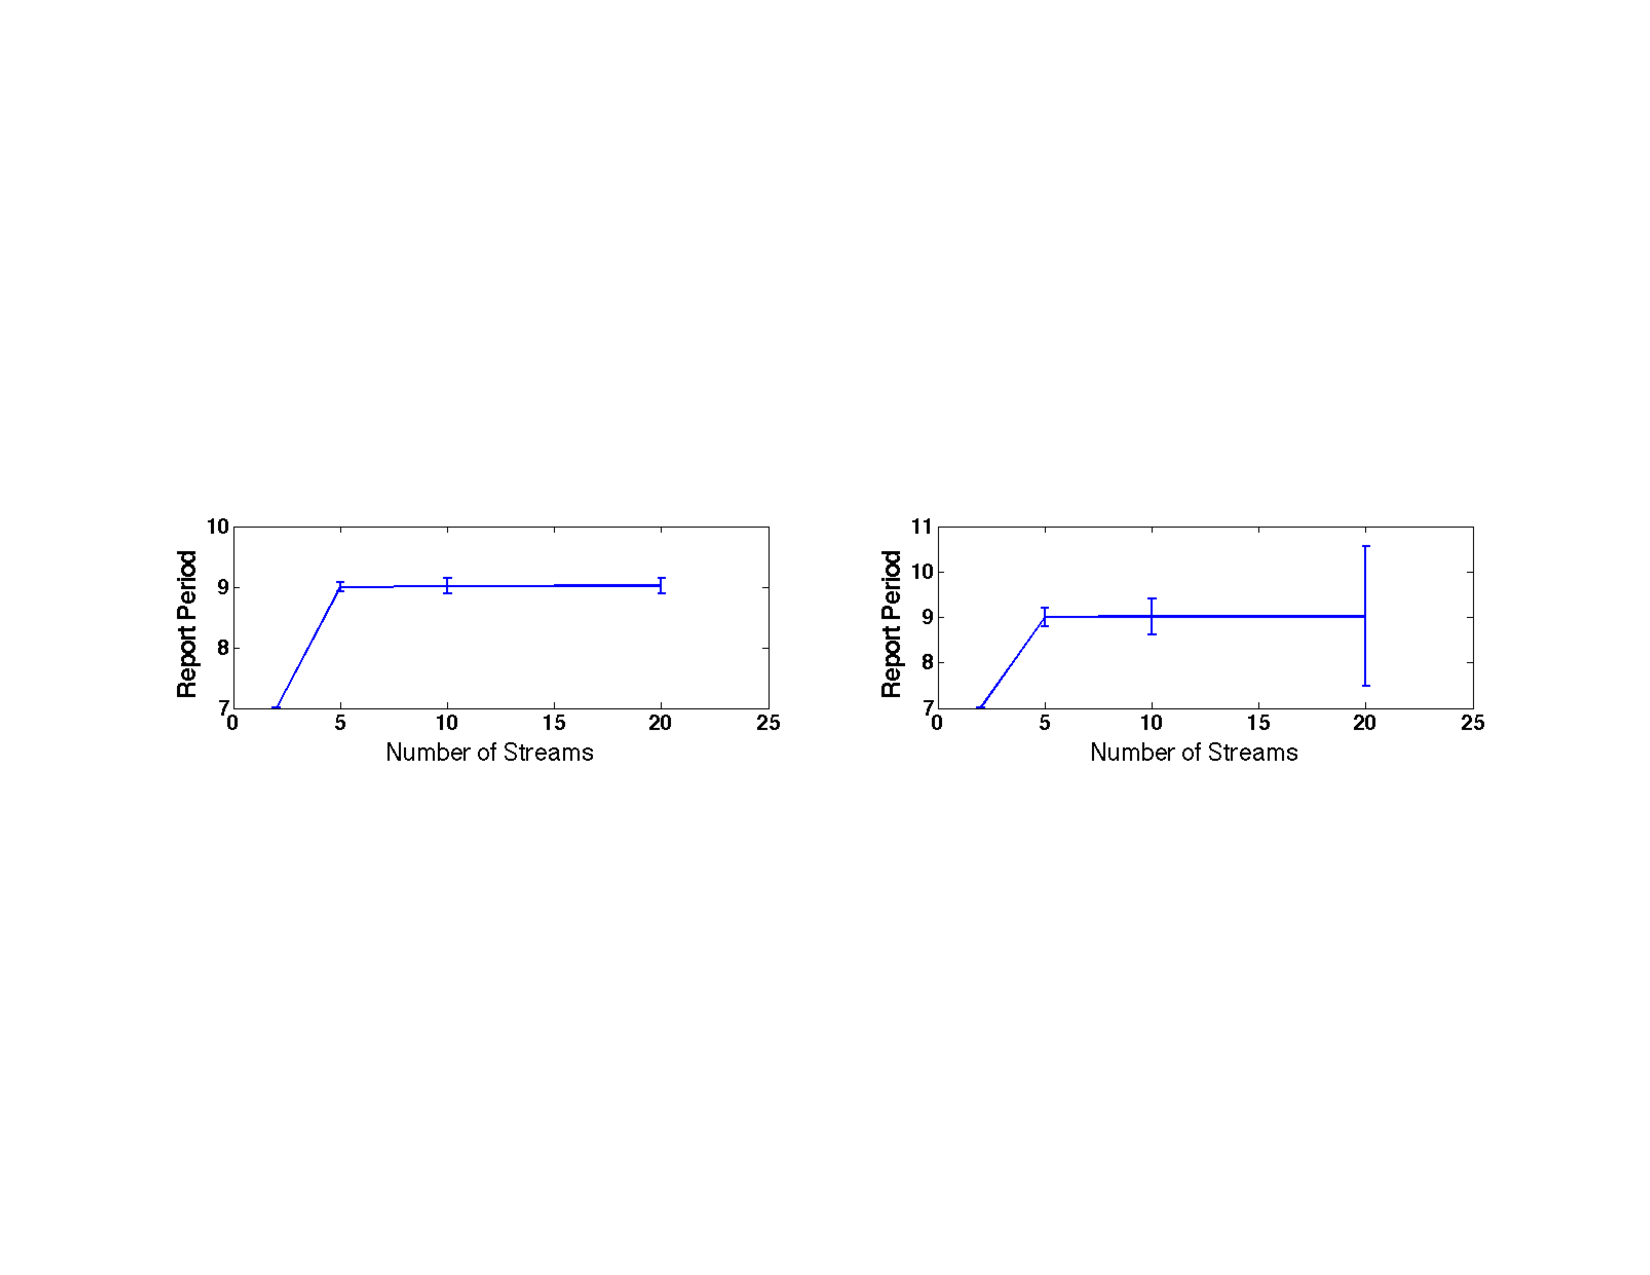
\includegraphics[width=1.0	\columnwidth]{figs/period_vs_streams}
\caption{}
\label{fig:report_periods}
\end{figure}

\section{Related Work}


\section{Summary}




% \chapter{Metadata Evolution and Verification}
% \section{Verication through Sensor Data}

% \section{Types of Verification}
% \subsection{Geometric Verification}
% \subsection{Functional Verification}
% \subsection{Value Verification}

% \section{Structural Verification With Empirical Mode Decomposition}

% \subsection{Introduction}
The United States leads the world in per-capita energy consumption.
Our electricity use has consistently increased over the last 40 years~\cite{oecd2011} and other parts of the world are rising all 
too rapidly.  With the specter of climate change and the increasing cost of energy, we must explore new
ways for individuals to gain visibility and insight into their energy consumption in order to optimize and reduce it. 
With the increasing penetration of embedded sensors in the environment and
the continued rise in smartphone adoption, we see an opportunity for smartphones to bridge the physical world
to our computational infrastructure and provide an `energy lens' on the physical world.  

We use mobile phones to construct an entity-relationship 
graph of the physical world and combine it with streaming sensor data in order to perform detailed energy-attribution.
We limit the scope of the world to a single building domain.  We have designed and implemented a real-time, mobile energy auditing
application, called the `Energy Lens', that allows us to collect information about 
things throughout the building and how they are related to each other.  For example, computer X is inside 
room Y and connected to meter Z.  Then, we use these relationships to guide our data look-up and analytical
calculations.  For example, the load curve of room Y consists of the sum of all the power traces for loads
inside room Y.  We use the mobile smartphone as the main input tool.  Our work examines \emph{three main challenges} in setting up and 
deploying a real, whole-building infrastructure to support real-time, 
fined grained energy analytics.  

The first challenge is related to tracking and mobility.
The use of mobile phones presents classical, fundamental challenges related to mobility.  Typically, mobility
refers to the phone, as the person carrying it moves from place to place.  However, in the energy-attribution
context, we are also referring to the movement of energy-consuming objects.  Tracking their relationships to spaces 
and people is as important as tracking people.  We describe how we deal with \emph{both moving people and 
moving objects} and show that these historically difficult problems can be addressed relatively easily, if the proper infrastructure is 
in place.  %We provide evidence that the approach is simple, incrementally deployable, and scalable.

The second challenge is about capturing the inter-relationship semantics and having these inform our  analytics.
We adopt the general notion of physical tags that identify objects in the world.  Our system uses \emph{QR codes} to tag things and locations 
in the physical world.  However, \emph{any tag that provides a unqiue identifier for an object could serve the same purpose}.
Once tagged, there are three types of interactions -- 
registration, linking, and scanning -- which establish important relationships.  Registration is the act of creating a virtual object 
to represent a physical one.  Linking captures the relationship between pairs of objects.  Scanning is the act of performing an item-lookup.
Each of these interactions requires a set of swiping gestures.  Linking requires two tag swipes while the other two actions
require a single tag swipe.  Internally, we maintain a \emph{entity-relationship graph (ERG)} of things, people, and locations, that gets
updated through these sets of gestures.

The third challenge is about indoor network connectivity and access.
In order to connect these components, we rely on having `ubiquitous' network connectivity.  However, in practice, network
\emph{availability} is intermittent and our system must deal with the challenges of intermittency.  We discuss how caching
and logging are used to address these challenges.  Moreover, when connectivity is re-established, we must deal with
applying updates to the ERG, as captured by the phone while disconnected.  
% Conflicts can also occur during an update.  For example, the two updates may disagree about which items are attached
% to which meters.  We implement a very simple conflict resolution scheme, described in section~\ref{sec:conflicts}.
% Finally, certain physical-state transitions are represented as a set of updates to the ERG that must be applied 
% atomically.  We implement transactions in the log-replay and transaction manager.
% Our `Energy Lens' system is deployed in a building on our campus.  We discuss
% its architecture and our design choices.  
  
% We also discuss novel strategies for tracking moving people/things and describe how we implement these in our system.  In summary, our work
% makes the following contributions:

% \begin{itemize}
% \item We design and implement a system that captures and combines physical entities, their inter-relationships, and real-time sensor data 
% 		in buildings.% using mobile phones, qr code, and a cloud-based infrastructure.
% \item We observe that certain combinations of swipes give us useful information to set the location of people and things over time.
% 		We codify this observation in our \emph{context-tracker} and use it to maintain consistency between the entity-relationship graph and the 
% 		state of the physical world.  To the best of our knowledge, this is radically different from the approaches in standard 
% 		localization techniques.  However, we argue that it can be used to \emph{enhance} their accuracy and overall performance.
% \item We implement a prefetching algorithm to obtain context-dependent information to both improve performance and
% 		enable disconnected operation.  We also design and implement a log-replay and transaction manager over our data management layer.  We describe how different conflict-resolution policies can be implemented and our rationale for the policies we chose.
% \end{itemize}

% \vspace{0.08in}

% In the next sections we go through a motivating scenario.  We then discuss some related work, followed 
% by the system architecture, evaluation, and future directions.

% \section{Related work}

%\begin{itemize}
% \item dashboard
% \item andrew's lightin control work
% \item Kamin's hvac control work
% \item BEMs
% \item sMAP stuff
%\item Buildsys 2010 work~\cite{hbci}
%\item distributed consistency management: COPS
%\item mobility: tracking things with RFID~\cite{rfid_gonz2006}
%\item mobility: tracking of people, wifi indoor localization
%\item entity-relationship graphs
%\item homeOS [microsoft]
%\item HP Cooltown~\cite{cooltown}
%\end{itemize}
Our work touches on several areas from smart home research to logistics.  In the building space, there has been
some interest in building various kinds of energy-related visual and control applications.
This work focuses on the object definition, tracking, and management component of the architecture proposed by 
Hsu et al.~\cite{hbci}.  Their work stratefied the set of challenges that one could potentially face if the application 
were deployed at scale.  Our
work, in constrast, bases its design rationale on a \emph{real deployment} that is taking place at scale in a building 
on our campus.  We focus on solving fundamental systems challenges in dealing with intermittent connectivity
and conflict resolution in tracking people and things over time.  We also focus on leveraging gestures to minimize
the cost of interaction for users, while maximizing the information we can attain about the state of the world.

% Tracking people/indoor localization
An important aspect of the Energy Lens is determining when people and things have moved.  This requires some form 
of indoor localization.  There's a large body of literature in the area of indoor localization with mobile phones ranging from 
using wifi~\cite{radar}, to sonar~\cite{cricket}, to ambient noise~\cite{abs}, and a combination of sensors on the 
phone~\cite{surroundsense, darwinphone}.  Dita~\cite{dita} uses acoustic localization of mobile phones and also uses the infrastructure 
to determine gestures in free-space that are classified into pre-defined control actions.  Each of these require relatively complex 
software and/or infrastrure.  
We take a radically different, simple approach.  We use cheap, easy to re/produce tags (QR codes), place them on things in the 
environment over incrementally and use the natural \emph{swiping gesture} that users make, when interacting with the Energy Lens 
application, to track when they have moved or when the objects around them have moved.  The working principal is to attain as much 
information from their gesture to determine when something/one has moved.  We discuss our heuristics in section~\ref{sec:swipes}.

% context-aware apps
ACE~\cite{ACE} uses various sensors on the phone to infer a user's context.  The context domain consists of a set of user activities
and semantic locations.  For example, if ACE can distinguish between {\tt Running, Driving, AtHome, or InOffice}.  ACE also infers 
the one from the others, so if the user is {\tt AtHome} then they are not {\tt InOffice}.  Energy Lens uses inference to determine
when a person or thing has moved.  Certain swipe combinations give us information about whether they moved and where they moved to or
whether an item moved and where it moved to.  The main difference is that we only infer context when a user is actively swiping, rather
than a continuous approach.  Pretching is a fundamental technique used in many domains.  However, the cost of a prefetch for mobile
application outways the benefits if the prefetched data is not useful.  Informed mobile pretching~\cite{IMP} uses cost-benefit analysis 
to determine when to prefetch content for the user.  In the Energy Lens context, we prefetch data based on their location swipes.
We also rely on pretching to anticipate loss of connectivity, not just to improve preformance.

% Tracking things
Logistic systems focus on the tracking of objects as the move through distribution sites to warehouses, stores, shelves,
and purchase.  Items are tracked through bar code or RFID readers.  However, the workload is very structured and well
defined.  The authors of~\cite{rfid_gonz2006} describe this structure and leverage it to minimize storage
requirements and optimize query-processing performance.  Energy Lens uses the QR codes as the tag and the phone as an active
reader.  As objects move, users scan those items to their new location.  However, objects may belong to one or
many people, they can be metered by multiple meters a day, and their history in the system
is on-going.  In contrast, a typical logistics workload has a start (distribution site) and end point (leaving the store
after a sale).  In our workload, relationship semantics are important; we need to know whether the meter is \emph{bound-to}
rather than simple \emph{attached-to} an item.  We discuss the difference later in the paper.
% In addition to traditional logistics-style queries -- \emph{What is the average time that it took coffee-makers to move from the 
% warehouse to the shelf and finally to the checkout counter in January of 2004?} -- energy-analytics requires queries to group
% partial traces from meter data by tracking what meters the item attached to over the specified time-frame.
% The Energy Lens system collects and manages this kind of information to enable such queries.
Furthermore, we take advatange of natural gestures the user makes with the phone while scanning QR codes to extract
information about the current location of the user or things.

% Tagging items, virtual services
The key idea in the HP Cooltown~\cite{bridgingphysical,cooltown} work is to web-enable `things' in the world, grouped-by
`place', and accessed by `people' via a standardized acquisition protocol (HTTP) and format (HTML, XML).  
Cooltown creates a web presence for things in the world either directly (embedded web server) or indirectly 
(URL-lookup tag) as a web page page that display the services it provides.  Many of the core concepts in Cooltown 
also show up in Energy Lens.  The main overlap is the use of tags in the world that contain a reference to a virtual 
resource, accessible via HTTP through
a network connection.  Cooltown, however, explicitly chooses not maintain a centralized relationship
graph, it leverages the decentralized, linking structure of the web to group associated web pages together.
Furthermore, things are assumed to not move.  People are the main mobile entities.  The kind of applications
we wish to support must track where things are and their specific inter-relationships.  We imposed a richer set of 
semantics on our, centrally maintained, relationship graph and use it to provide detailed energy information.


% \section{Dataset}
The data we used was obtained from a deployment of sensors in a 12-story office building
on the campus of the University of Tokyo~\cite{gutp, ogawa:lncs2011}.  The deployment consists of 
almost 700 sensors monitoring device power consumption, ranging from plug-load devices to components of the
heating, ventilation, and air conditioning system (HVAC) and lighting.  Sensors also reported temperature, 
pressure, device-state, and other information.  Each sensor reports data on the
order of minutes.  Over 500 GBs of data was collected over a 2-year span.

\begin{figure*}[tb]
\hspace{-2cm}
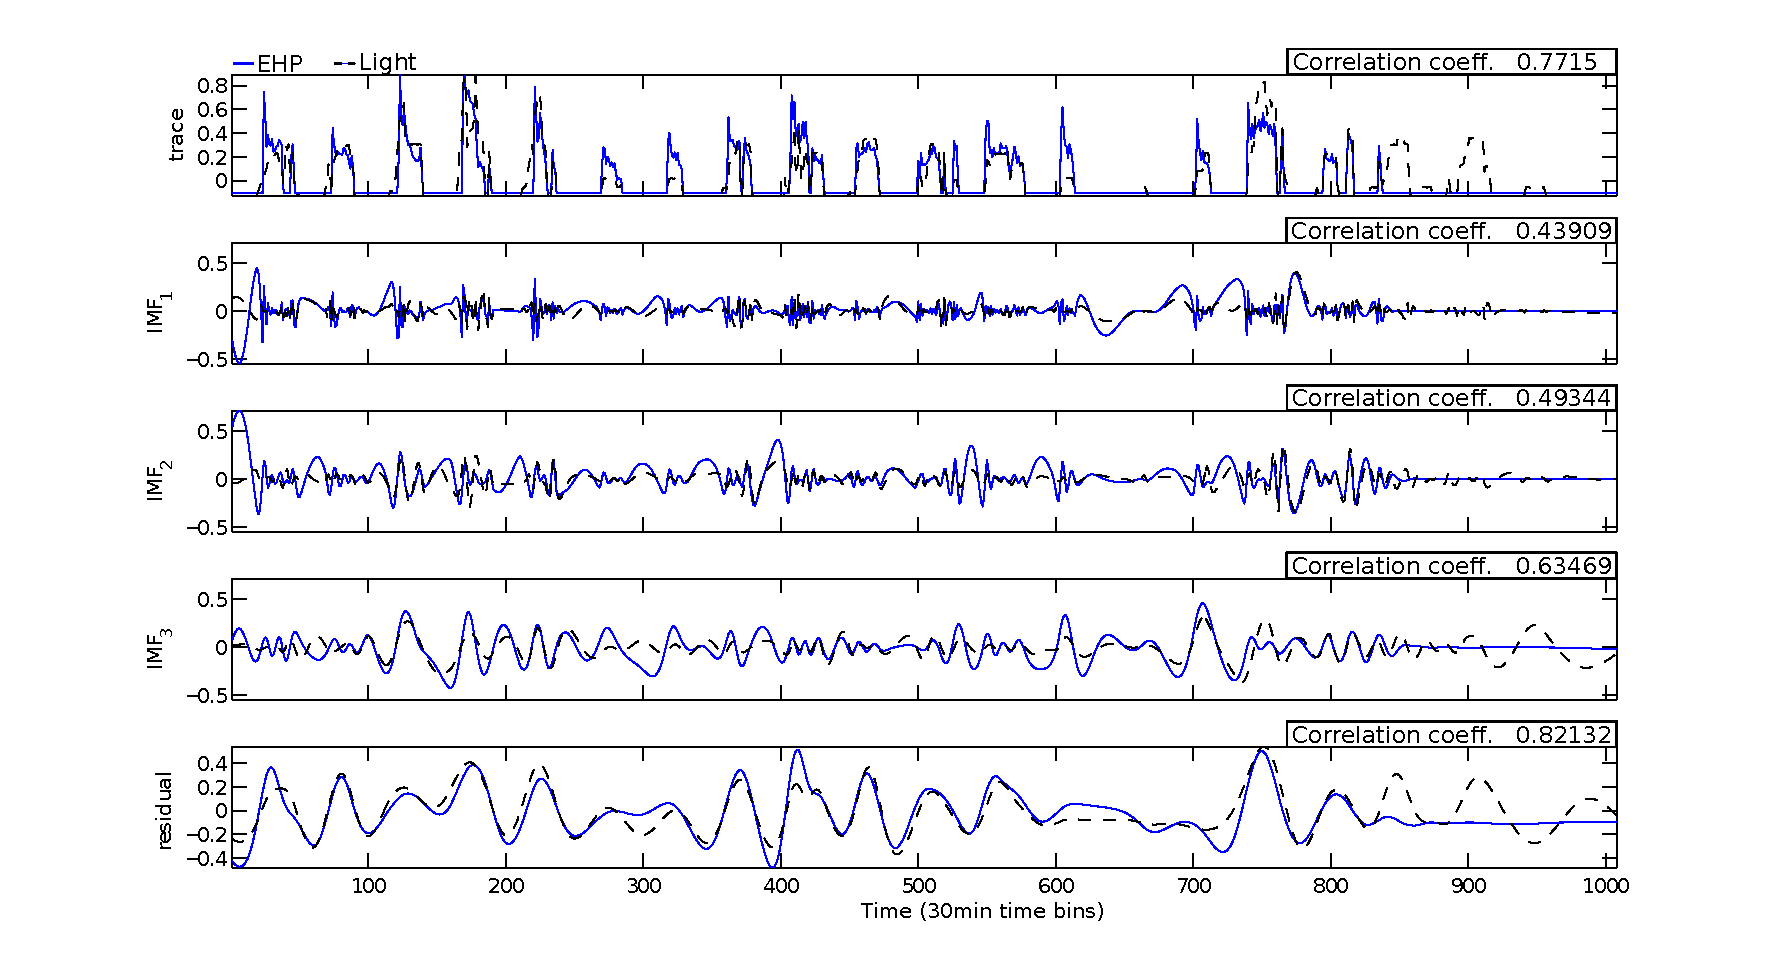
\includegraphics[width=1.2\textwidth]{img/emd_25_26-eps-converted-to}
\vspace{-1cm}
\caption{Decomposition of the EHP and light trace using bivariate EMD. IMFs correlation coefficients highlight the intrinsic relationship of the two traces.}
\label{fig:emd}
\end{figure*}

% The intent of the Green University of Tokyo Project (GUTP) \cite{gutp} is to reduce the university environmental impacts associated to its electric energy consumption.
% The first step of this project was to deploy sensors at the Building No.2 of the Faculty of Engineering 
% Electric power consumption of a 12 floors building containing researchers office and classroom.
% 1215 sensors monitoring different devices...

%received attention in the past \cite{ogawa:lncs2011}.

For this investigation, we focus on a three-week span in the summer of 2011 (from July 4th to July 24th).
The dataset captures regular work days, weekends, and one holiday (July 18th).  This timeframe captures
the typical usage of the equipment, triggered by occupant activity.  For the initial
analysis, we focus on three sensors; two water pumps and a light feed.  The first pump is an 
``electric heat pump'' and is labled as EHP, the second  is a ``gas heat pump''
and labeled as GHP.  The room lighting system serves the same room as the EHP.  The GHP
serve a different room on the same floor.  The expanded portion of our analysis pivots as the EHP
and does a pairwise comparison between it and all other sensors in the building.

% includes one day holiday (July 18th)
% 3 different sensors:
% \begin{itemize}
%  \item Two are measuring the electric power consumption of two devices from the same room; an electric heat 
%  		pump (EHP) and the room lighting system.
%  \item One is measuring the electric power consumption of a gas heat pump (GHP) that is pumping water to cool 
%  		a different room in the same building.
% \end{itemize}

% Later we expand our analysis to include all the sensors in the building.


\section{Problem statement and Initial approach}\label{problem}
% In our analysis, we are focused on finding devices that are correlated in their use over time.  Therefore, the
% main objective is to examine how device traces relate to one another.  The wish to identify
% correlated device-trace patterns at large spatio-temporal scales.

In buildings, metadata is poorly and unsystematically managed within a single system domain.  Moreover, 
with the ever growing number of additional sub-meters, it is important to quickly integrate
sensor data from multiple systems to understand the full state of the building.  It is also important to 
understand how sensors are used in concert.  Anamolies in usage may indicate underlying problems with 
the equipment or inefficient/incorrect usage.  

We begin our analysis by running direct correlation between the traces.
Figure \ref{fig:raw} shows the raw traces for the three devices discussed in 
the previous section (EHP, GHP, light).  All three exhibit a diurnal usage pattern.  On weekends, each
draw less power.  The correlation coefficient for 
 the EHP and light is $0.7715$ and the correlation coefficient for the EHP and GHP is $0.6370$.
Running correlation across them yields high correlation coefficients, mostly
due to their underlying daily usage pattern.

% Usual measures on sensor data like correlation coefficient or granger causality \cite{kim:buildsys2010}
% -- this is not working

\begin{figure}[t!]
\centering
 \subfigure[EHP trace]{\label{fig:raw_ehp}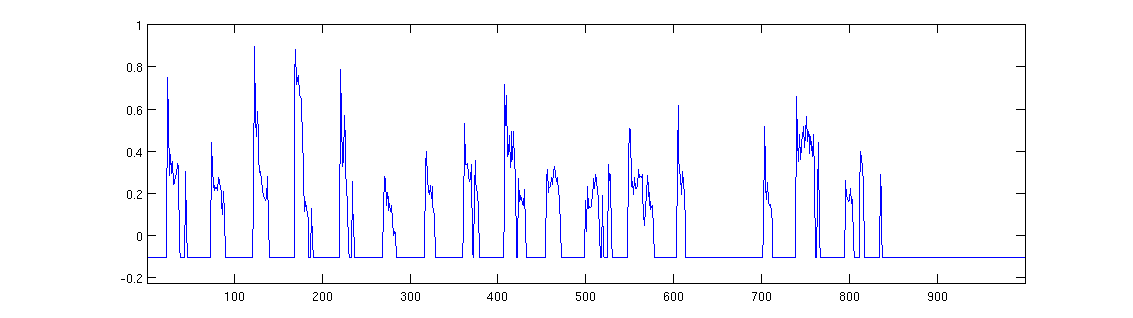
\includegraphics[width=.4\textwidth]{img/25.png}}
 \subfigure[Light trace]{\label{fig:raw_light}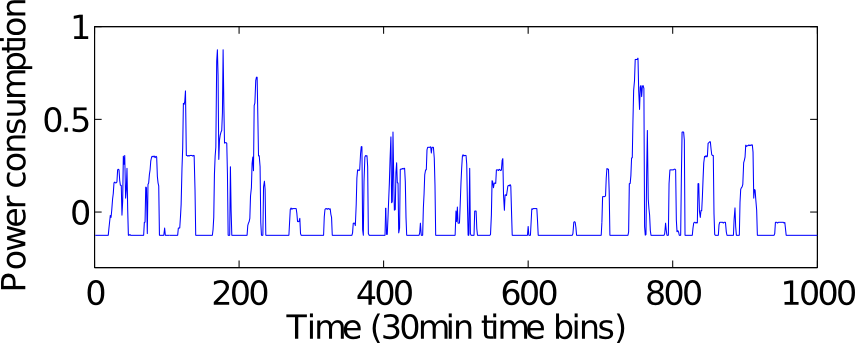
\includegraphics[width=.4\textwidth]{img/26.png}}
 \subfigure[GHP trace]{\label{fig:raw_ghp}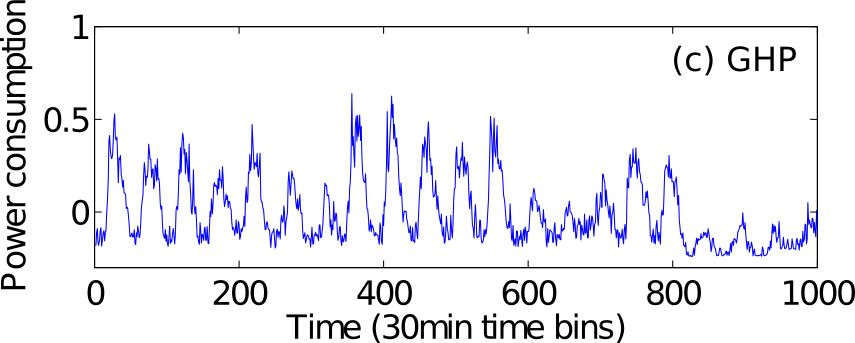
\includegraphics[width=.4\textwidth]{img/41.png}}
 \caption{Traces from three different sensors captured in 2011 from July 4th to July 24th. Data is normalized and aggregated into 30 minutes time bins.}
 \label{fig:raw}
\end{figure}

% For example correlation coefficients for the 3 signals...
% correlation coefficient for the EHP and Light signals: $0.772013$
% correlation coefficient for the EHP and GHP signals: $0.636967$

% These scores suggest that the EHP signal is related to the two other measured signals.

% These results were expected for the EHP and light traces, as the two measured devices operate for the same room 
% and are used simultaneously.  More importantly, they are used to support the occupants of the rooms they are serving.
% We were somewhat surprised by the magnitude of correlation between the pumps, since they serve rooms on
% opposite sides of the building and operate independently.  However, occupancy and weather patterns are similar,
% and the underlying trend is captured by the correlation calculation.
% The difference between the correlation coefficients is small and one might conclude that all three are
% closely related to one another.  That conclusion is not false but misleading.  Correlation on the raw 
% traces is sensitive to the underlying trend shared by the traces.  In order to meaningfully distinguish between
% truly related devices we need to remove the common trends. 

Our initial results were not surprising.  The diurnal pattern dominates the comparison between the sensors.
Weather is the main driver for this behavior and it affects the readings in almost all of the
sensors in our dataset.  Cross-correlation on raw sensor data is insufficient for filtering intrinsically related
behavior.  Upon closer examination of the data we assess the following:

\begin{itemize}
\item The main underlying diurnal trend occurs in almost all the traces.
\item Occupancy and room activities occur at random times during the day and change 
		at a higher frequency than weather patterns.
\item Sensors that serve the same location observe the same activities.  Therefore, their underlying
		measurements should be correlated.
\end{itemize}

In order to uncover these relationships we must remove low-frequency trends in the traces and
compare the readings at high frequencies.

% \begin{table}
% \begin{center}
% \begin{tabular}{|l|l|l|l|l|l|}
% \hline
% × & Raw trace & 1st IMF & 2nd IMF & 3rd IMF & Residual\\ \hline
% EHP, Light & 0.7715 & 0.43909 & 0.49344 & 0.63469 & 0.82132 \\ \hline
% EHP, GHP & 0.6370 & 0.0060274 & 0.063546 & 0.16764 & 0.79378 \\ \hline
% \end{tabular}
% \caption{Correlation coefficients of the analyzed trace and their IMFs uncovered by EMD}
% \label{tab:corr}
% \end{center}
% \end{table}
% \subsection{Simple Scenario}

\begin{figure*}[tb]
\hspace{-2cm}
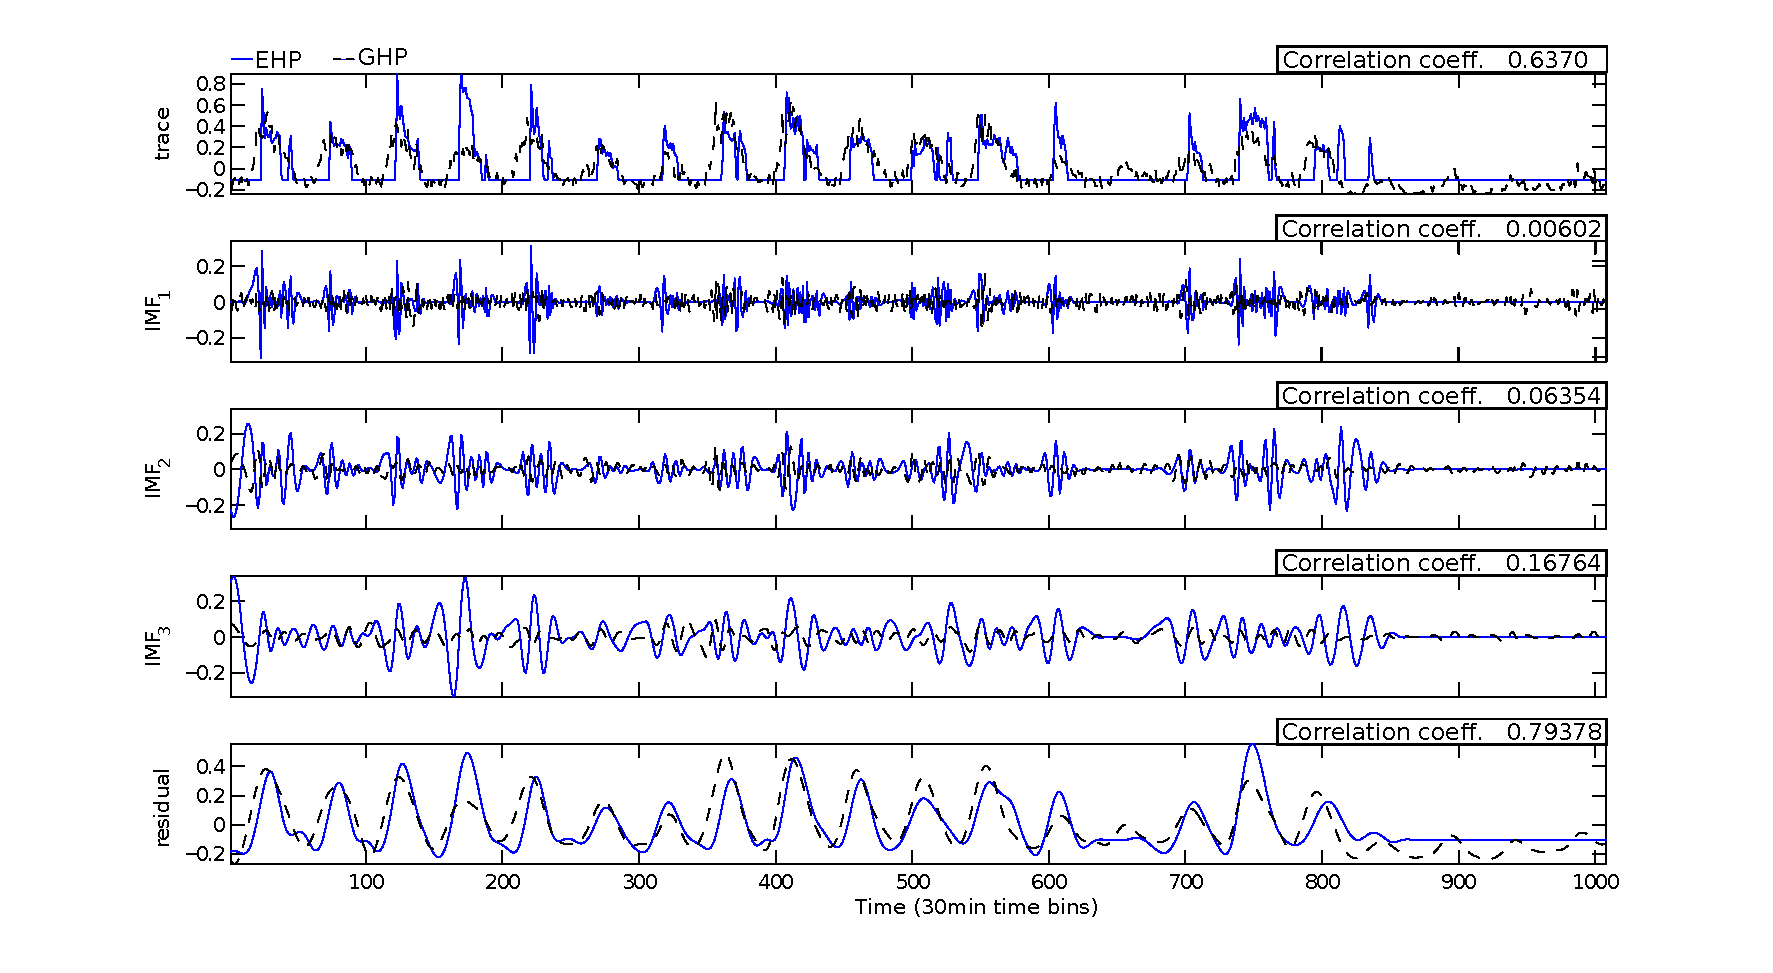
\includegraphics[width=1.2\textwidth]{img/emd_25_41-eps-converted-to}
\vspace{-1cm}
\caption{Decomposition of the EHP and GHP trace using bivariate EMD. IMFs correlation coefficients highlight the intrinsic independence of the two traces.}
\label{fig:emd2}
\end{figure*}

% The small difference between the two computed correlation coefficients is misleading as one could conclude that the three signals are correlated and the corresponding devices are activated by a single action.

% The high correlation coefficients obtained for these three signals result .... weekly pattern....
% small difference = local fluctuation...

% this high score comes from the fact that the two devices are monitoring offices that are weekly used.

% Indeed the weekly pattern of the data trump the correlation coefficients....

% How to inspect only the local fluctuations...?
% we'd like to have an elegant solution (i.e. not specifying the interesting time scale)


% \section{Methodology}\label{method}
%Remove the weekly trend of the data to analyze the detailed changes that convey the device behavior at small time scales.

% Our initial approach examined correlation analysis on raw sensor traces.  However, we quickly
% found that correlation is overly sensitive to fluctuations in the data.
Fundamentally, the readings are driven by the same underlying phenomena: 
weather and occupancy.  Weather influences \emph{all} the data similarly.  Occupancy, however, changes
throughout the building and should be used as a differentiating component in the signal
comparisons.  Sensors that share spatio-temporal elements should be correlated after the removal
of the underlying trend driven by the weather.  In order to find unique relationships we needed to remove 
this common trend.

\subsection{Empirical Mode Decomposition}
Empirical Mode Decomposition (EMD) \cite{huang:emd1998} is a new techniques used for de-trending data.
Specifically, EMD detrends non-stationary, non-linear timeseries data.  A trend is defined as 
an intrinsically determined monotonic function within a certain temporal span or a function in which there 
can be at most one extremum within that temporal span.  A non-stationary signal is a signal whose mean and
variance change over time.  EMD is a process, rather than a theoretical tool.

We describe the process as follow:  for a signal \emph{X(t)}, let $m_1$ be the mean of its upper and
lower envelopes as determined from a cubic-spline interpolation of local maxima and minima. The locality 
is determined by an arbitrary parameter.

\begin{enumerate}
\item The first component $h_1$ is computed: $h_1=X(t)-m_1$
\item In the second sifting process, $h_1$ is treated as the data, and $m_{11}$ is the mean of $h_1$'s upper and lower envelopes: $h_{11}=h_1-m_{11}$
\item The procedure is repeated $k$ times, until $h_{1k}$ is a function: $h_{1(k-1)}-m_{1k}=h_{1k}$
\item Then it is designated as $c_1=h_{1k}$, the first functional component from the data, which contains the shortest period component of the signal. We separate it from the rest of the data: $X(t)-c_1 = r_1$, and the procedure is
repeated on $r_j: r_1-c_2 = r_2,\dots,r_{n-1} - c_n = r_n$
\end{enumerate}

The result is a set of functions called intrinsic mode functions (IMF); the number of functions in 
the set depends on the original signal~\cite{emd_process}.  An IMF is any 
function with the same number of extrema and zero crossings, with its envelopes being symmetric with respect to zero.
We run our correlation analysis on the shared IMF outputs between a pairs of signals.  In order to ensure 
that the IMFs corresponding to two distinct signals are on the same time scale, we use 
bivariate EMD \cite{rilling:biemd2007} to decompose two signals at once. The main use of EMD is for removing dominant trends to conduct a meaningful spectral analysis of the data.


% \subsection{Results}

We test our hypothesis in this section by using EMD to remove low-frequency trends in the data
and run correlation calculation at overlapping IMF timescales.  We discover that EMD allows us
to find and compare high-frequency instrinsic behavior that is spatially correlated across
sensors.  We begin with a small set of three sensors (EHP, GHP, light) and expand our scope
to include all the sensors in the dataset.



\subsubsection{Initial analysis}
Lets consider the simple example of Section \ref{problem} where we would like to know if the EHP trace is correlated with the two other traces.
Recall that the correlation coefficients of the raw feeds was $0.7715$ and $0.6370$, corresponding to the light 
and GHP, respectively.
As stated in previous section this result is correct but not so meaningful, since most of the traces
display the same diurnal pattern.
Figure \ref{fig:emd} and Figure \ref{fig:emd2} show the EMD decomposition of the three traces.
For each trace, EMD has retrieved three IMFs that highlight the higher frequencies of the traces.

Figure~\ref{fig:emd} shows the normalized raw trace (top) and EMD output IMFs and residual as well as the 
correlation coefficients calculated on the IMFs for the EHP and
light traces.  The correlation coefficients are $0.43909$, $0.49344$ and $0.63469$ corresponding to the IMF1, 
IMF2, and IMF3, respectively.  Notice the high correlation between the high-frequency IMFs.
We know that the light and EHP serve the same room, and their high-frequency IMF correlation corroborates
our prior knowledge.
Figure~\ref{fig:emd2} shows a complementary result, for the EHP and GHP comparison.
The correlation coefficients for the EHP and GHP IMFs suggest that the two may be independent.  In fact, they
\emph{are} indepdent; they serve completely different rooms in the building!

EMD allows us to remove low-frequency trends that add noise to the original analysis.
By comparing IMFs, we see both intrisically correlated and \emph{uncorrelated} behavior.  In the next
section we expand our analysis and show the effectiveness of our methodology. 
% Although promising, these results must be validated across the rest of the
% dataset to confirm their significance.  


\subsubsection{Validation}
To validate the effectiveness of our approach, we analyze the same three-week time span for \emph{all} 674 
sensors deployed in the building.
For each trace $S$ we compute two scores: (1) the correlation coefficient between $S$ and the EHP trace
and (2) the average value of the IMF correlation coefficients.

\begin{figure}[tbh!]
\centering
 \subfloat[Raw traces correlation coefficients]{\label{fig:histo1}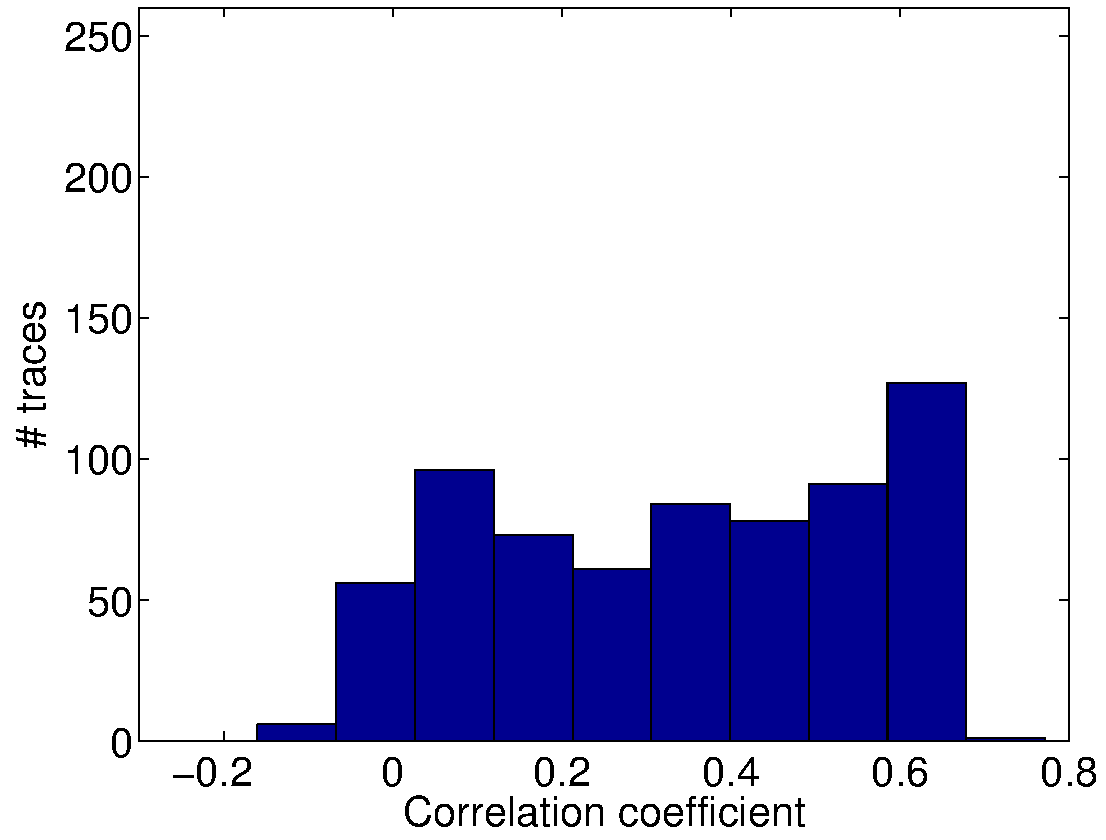
\includegraphics[width=.43\textwidth]{figs/allFloors_week1_week4_corr_abs-eps-converted-to}}
 \subfloat[Average IMFs correlation coefficients]{\label{fig:histo2}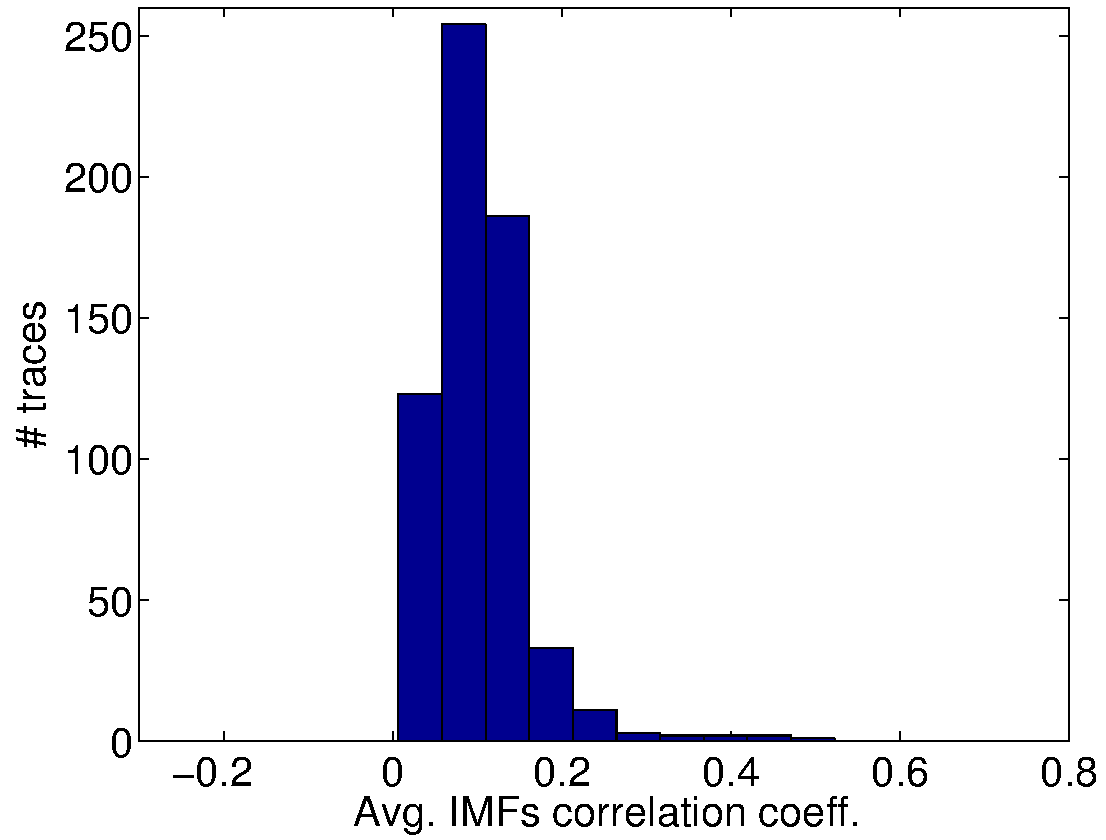
\includegraphics[width=.43\textwidth]{figs/allFloors_week1_week4_emd_abs-eps-converted-to}}
 \caption{Distribution of the correlation coefficients of the raw traces and correlation coefficients average of the corresponding IMFs using 3 weeks of data from 674 sensors.}
\label{fig:histo}
\end{figure}

\begin{figure}
\centering
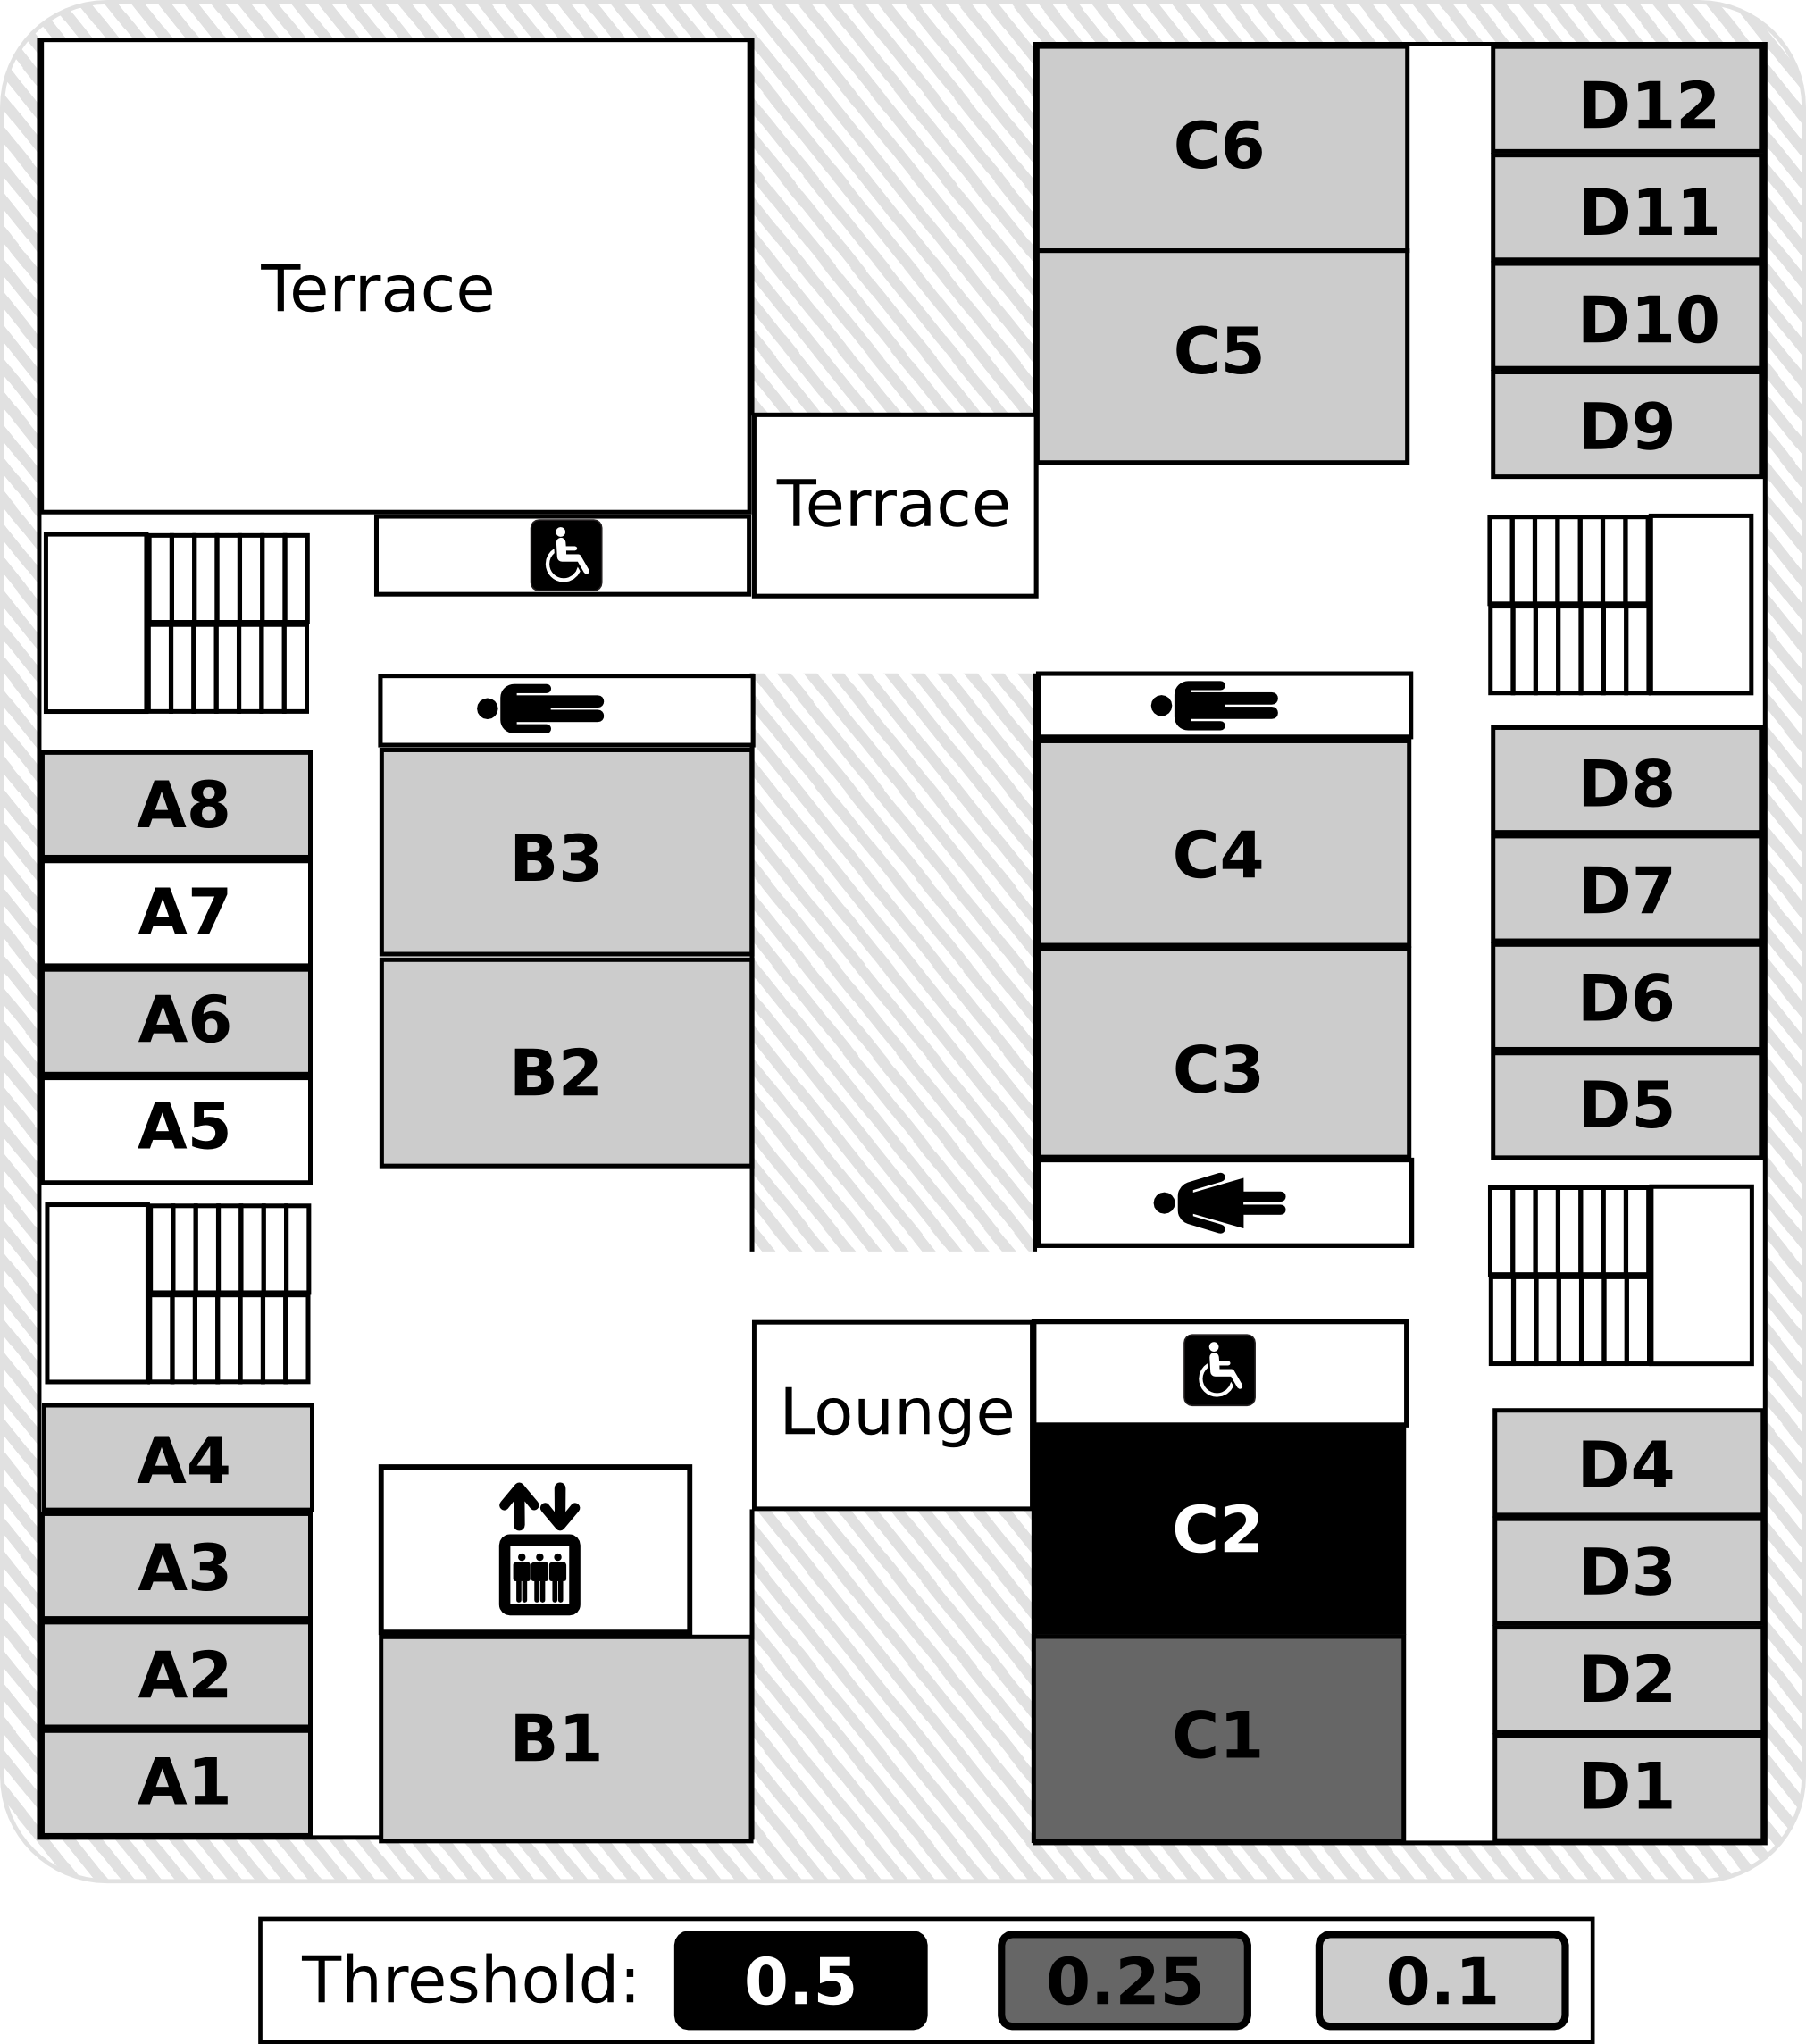
\includegraphics[width=.45\textwidth]{figs/floorMap.png}
\caption{Map of the floor where the analyzed EHP serves (room $C2$). The location of the sensors identified as related by the proposed approach are highlighted, showing a direct relationship between IMF correlation and spatial proximity.}
\label{fig:map}
\end{figure}

Figure \ref{fig:histo1} shows the distribution correlation coefficients.  Notice
that a large fraction of the dataset is correlated with the EHP trace.
\emph{Half} the traces have a correlation coefficient higher than $0.36$.  As expected, the underlying
trend is shared by a large number of device.
Although the highest score (i.e. $0.7715$) corresponds to the light in the same room that the EHP serves,
there are 118 pumps, serving all areas of the building, with a correlation higher than $0.6$.
Using only these results, it is not clear where the threshold should be set.  The distribution is close to 
uniform, making it difficult to 
know of how well your threshold discriminates against unrelated traces.
% Moreover, the distribution of the traces is almost uniform, thus, discriminating correlated traces is a laborious task.

Figure \ref{fig:histo2} shows the distribution of the average correlation value for the IMFs of
each trace and the EHP.  The number of traces correlated in the high frequency IMFs is significantly smaller
than the previous results. It's clear from the distribution that only a small set of devices are
\emph{intrinsically correlated} with the EHP.  In fact, \emph{only 10 traces out of 674} yielded a score higher than 
$0.25$. This allows us to easily rank traces by correlation.

Upon closer inspection of the 10 most correlated IMF traces, we find that there is a spatial relationship
between the EHP and the ten devices.  In fact, there is a direct relationship between score and distance from
the areas served by the EHP.  Figure~\ref{fig:map} shows a map of the floor that contains the rooms served by this
EHP.  The EHP directly serves room $C2$.  We introduce a correlation threshold to cluster correlated traces by score.
We highlight rooms by the threshold setting on the IMF correlation score.
When we set the threshold at $0.5$ we see that the sensors that have a correlation higher fall within room $C2$ --
the room served directly by the EHP.  As we relax the threshold, lowering it to $0.25$ and $0.1$ we see radial expansion from $C2$.  The trace with the highest score, $0.522$, is the trace corresponding to the lighting system \emph{in
the same room}.
The two highest scores for this floor (i.e. $0.316$ and $0.279$) are the light and EHP traces from next door, room $C1$.
Lower values correspond to sensors measuring activities in other rooms that have no specific relationship to the analyzed trace.  The results show a direct relationship between IMF correlation and spatial proximity and \emph{supports our initial
hypothesis}.


% Interestingly, the IMFs correlation coefficients reveal the spatial correlation of the sensors.
% Figure \ref{fig:map} is the map floor where the EHP trace is measured.
% Specifically, the EHP reports heating activity in the room $C2$.
% in the simple scenario the GHP is located in the room A5.



% \subsection{Limitations}
EMD is useful for finding underlying behavioral relationships between traces of sensor data.  However,
when we set the timescales smaller than a day, the results were not as strong.
The trace has to be long enough to capture the trend.  For this data set, the underlying
trend is daily, therefore it requires there to be a significant number of samples over many days.
%  to
% for this method to be effective.
Although this was a limitation for this dataset, it really depends on the underlying phenomenon that
the sensors are measuring.  Its underlying trend is ultimately what EMD will be able to separate
from the intrinsic modes of the underlying signal.

\subsection{Discussion}
EMD allows us to effectively identify fundamental relationships between sensor traces.
% Using EMD to find fundamental relationships between sensor traces effectively identifies intrinsically
% related behavioral relationships.
% was quite promising for building
% up models of correlated usage.  
We believe that identifying meaningful usage-correlation patterns can help reduce oversights
by the occupants and faults that lead to energy waste.  A direct application of this is the identification
of simultaneous heating and cooling~\cite{simheatcool}.  Simultaneous heating and cooling is when heating
and cooling system either compete with one another or compete with the incoming air from outside and is
a cause for major energy waste in building~\cite{simheatcool}.  The longer it goes undetected,
the more waste there is.  However, it is very difficult to identify since the occupants do not notice
changes in temperature.  Our analysis can be used to build a correlation model between the outside
heating cooling temperature, the cooling coil temperature, and the outside air vent position.  If their behavior
is not correlated as expect, an alarm should be raised.

We can also apply it to other usage scenarios.  In our traces, for example, we found an instance where the pump
was on, but the lights were off.  The two are typically correlated, however, in this case they were not.
The air conditioning was pumping cool air into a room without occupants.
With our approach this could have been identified and corrected.  In future work, we intend to
package our solution to serve these kinds of applications.

% EMD works perfectly although the weekly pattern of the data is altered the last analyzed week.

% EMD inherently finds the interesting time scales.

% number of zero crossing = mean frequency/time scale:
%   TODO give the time scale for each IMF.


\section{Conclusion}
% what is our problem

% what we did

% contributions and main results

% future work


This paper set out to examine the underlying relationship between sensor traces to find interesting correlations
in use.  We used data from a large deployment of sensors in a building and found that direct correlation analysis on the raw
traces was not discriminatory enough to find interesting relationships.  Upon closer inspection, we noticed that
the underlying trend was dominating the correlation calculation.  In order to extract meaningful behavior this trend has
to be removed.  We concluded that empirical mode decomposition is a helpful analytical tool for de-trending 
non-linear, non-stationary data; inherent attributes contained by our traces.

We re-ran our analysis on the same traces, except we correlated the IMF outputs of the EMD operation on each of the traces and found that the pump was closely related to the lights in the same room served by the pump and
uncorrelated with a pump on the same floor serving a different room.  In order to corroborate the applicability
of our approach, we compared the pump trace with \emph{all} 674 sensor traces and found a strong correlation
between the relative spatial position of the sensors and their IMF correlations.  The most correlated IMFs were 
serving the same
area in the building.  As we relax the admittance criteria we find that the spatial correlation expands radially from
the main location served by the reference trace.

We plan to examine the use of this method in applications that help discovery changes in underlying relationships over time
in order to identify opportunities for savings in buildings.  We will use it to build inter-device correlation models
and use these models to establish ``normal'', ``abnormal'' usage patterns.  We hope to take it a step further and include a
supervised learning approach to distinguish between ``efficient'' and ``inefficient'' usage patterns as well.









% \section{Functional Verification through Classification and Experimentation}

% \section{Value-Based Verification Through Physical-Model Checking}

% \section{Related Work}

